%-------------------------------------------------------------------
% bachelor thesis - presentation
%
% topic: ACDC4JS - How to analyze a JavaScript garbage collector
%
% create by: Mario Preishuber
% create date: 2014, Jan 01.
%-------------------------------------------------------------------

\documentclass[xcolor=x11names,compress]{beamer}

\usetheme[pageofpages=of,
          alternativetitlepage=true,
          titlepagelogo=../imgs/uni_sbg_logo_sw.pdf,
		  ]{Mp}
\usepackage[american,austrian]{babel}  % language support
\usepackage{graphicx}
\usepackage{listings}
\usepackage{color}
\usepackage{color}

\definecolor{verylightgrey}{HTML}{EEEEEE}
\definecolor{lightgrey}{HTML}{DDDDDD}
\definecolor{darkgrey}{HTML}{999999}
\definecolor{blue}{HTML}{009EE0}
\definecolor{green}{HTML}{97BE0D}
\definecolor{orange}{HTML}{F29400}

\lstdefinelanguage{JavaScript}{
	keywords={
				break, case, catch, continue, debugger, default, delete, do, else, 
				finally, for, function, if, in, instanceof, new, return, switch, 
				this, throw, try, typeof, var, void, while, with
				},
	keywordstyle=\color{blue!70!black}\ttfamily,
	ndkeywords={class, export, boolean, throw, implements, import, this},
	ndkeywordstyle=\color{green!70!black}\ttfamily,
	identifierstyle=\color{black}\ttfamily,
	stringstyle=\color{orange}\ttfamily,
	sensitive=false,
	comment=[l]{//},
	morecomment=[s]{/*}{*/},
	commentstyle=\color{darkgrey}\itshape,
	stringstyle=\color{orange!90!black}\ttfamily,
	morestring=[b]',
	morestring=[b]",
	belowcaptionskip=1\baselineskip,
	breaklines=false,
	extendedchars=true,
	frame=none,
	frameround=tttt,	% or values t or f
	backgroundcolor=\color{white},
	showstringspaces=false,
	showspaces=false,
	showtabs=true,
	captionpos=b,
	numbers=left,
    numberstyle=\footnotesize,
    numbersep=9pt,
    tabsize=2,
}
\uselanguage{american}

\graphicspath{
	{../imgs/}
	{../imgs/plots/}
}


\title{ACDC4JS}
\subtitle{How to analyze a JavaScript garbage collector}
\author{Mario Preishuber}
\institute[]{Department of Computer Sciences \ University of Salzburg}
\date{January 13, 2014}

\begin{document}
	\begin{frame}
		\titlepage
	\end{frame}

	% \begin{frame}
	% 	\frametitle{Content}
	% 	%\setcounter{tocdepth}{1}
	% 	%\tableofcontents
	% 	\begin{itemize}
	% 		\item Performance analysis
	% 		\item JavaScript memory management benchmark
	% 		\item Experiments
	% 	\end{itemize}
	% \end{frame}

	%-----------------------------------------------------------------------
	% SECTIONS
	%-----------------------------------------------------------------------
	%-------------------------------------------------------------------
% bachelor thesis - presentation
%
% topic: ACDC4JS - How to analyze a JavaScript garbage collector
%
% create by: Mario Preishuber
% create date: 2014, Jan 01.
%-------------------------------------------------------------------
\section{Related work}	
\begin{frame}
	\frametitle{Related work}
	ACDC: Towards a Universal Mutator for
	Benchmarking Heap Management Systems \\

	\bigskip

	\textbf{Authors} \\
	Martin Aigner \\ 
	Christoph Kirsch \\

	\bigskip

	% What does ACDC stands for?
% 	\begin{itemize}
% 		\item \textbf{AC} periodic memory allocation and deallocation
% 		\item \textbf{DC} persistent memory
% 	\end{itemize}	
\end{frame}	
	%-------------------------------------------------------------------
% bachelor thesis - presentation
%
% topic: ACDC4JS - How to analyze a JavaScript garbage collector
%
% create by: Mario Preishuber
% create date: 2014, Jan 01.
%-------------------------------------------------------------------
\section{Introduction}	
	\subsection{Memory management}
	\begin{frame}
		\frametitle{Memory management}
		\begin{columns}
			\begin{column}{.1\linewidth}
				\includegraphics<1>[width=5.5em]{../imgs/memory_0.pdf}
				\includegraphics<2>[width=5.5em]{../imgs/memory_1.pdf}
				\includegraphics<3>[width=5.5em]{../imgs/memory_2.pdf}
				\includegraphics<4>[width=5.5em]{../imgs/memory_3.pdf}
				\includegraphics<5>[width=5.5em]{../imgs/memory_4.pdf}
				\includegraphics<6>[width=5.5em]{../imgs/memory_5.pdf}
				\includegraphics<7>[width=5.5em]{../imgs/memory_6.pdf}
				\includegraphics<8>[width=5.5em]{../imgs/memory_6.pdf}
				\includegraphics<9>[width=5.5em]{../imgs/memory_6.pdf}
			\end{column}
			\begin{column}{.7\linewidth}
				\begin{itemize}
					\item Typical memory structure
					\begin{enumerate}
						\item Program code
						\item Constants (e.g. strings) 
						\item Heap
						\item Stack
					\end{enumerate}
				
					\pause
					\pause
					\pause
					\pause
					\pause
					\pause
					\pause
					
					\item Memory management in C
					\begin{itemize}
						\item \textbf{Allocation} explicit with \texttt{malloc()}
						\item \textbf{Deallocation} explicit with \texttt{free()}
					\end{itemize}
		
					\pause
		
					\item Memory management in JavaScript
					\begin{itemize}	
						\item \textbf{Allocation} explicit / implicit
						%\begin{itemize}
						%	\item explicit with \texttt{new}
						%	\item implicit with initialization 
						%\end{itemize}
						\item \textbf{Deallocation} implicit %with destroying references
					\end{itemize}
				\end{itemize}
			\end{column}
		\end{columns}
	\end{frame}
	
	\begin{frame}[fragile]
		\frametitle{Memory management}
		\begin{footnotesize}
			\begin{lstlisting}[language=JavaScript]
				// C
				char *s = malloc(4*sizeof(char)); // explicit allocation
				strncpy(s, "abc\0", 4);
				...
				access(s);
				...
				free(s);                          // explicit deallocation
			\end{lstlisting}			
			
			\pause
			
			\begin{lstlisting}[language=JavaScript]
				// JS
				function dosomething() {
				  var s = "abc";                  // implicit allocation
				  ...
				}                                 // destroy references 
				
				dosomething();
			\end{lstlisting} %(unreachable implicit deallocation)
		\end{footnotesize}		
	\end{frame}
	
	\begin{frame}
		\frametitle{Memory management}
		\begin{center}
			\includegraphics<1>[width=25em]{../imgs/app_gc_1.pdf}
			\includegraphics<2>[width=25em]{../imgs/app_gc_2.pdf}
			\includegraphics<3>[width=25em]{../imgs/app_gc_3.pdf}
			\includegraphics<4>[width=25em]{../imgs/app_gc_4.pdf}
			\includegraphics<5>[width=25em]{../imgs/app_gc_5_a.pdf}
			\includegraphics<6>[width=25em]{../imgs/app_gc_6_a.pdf}
			\includegraphics<7>[width=25em]{../imgs/app_gc_7.pdf}
			\includegraphics<8>[width=25em]{../imgs/app_gc_0.pdf}
		\end{center}
	\end{frame}
	
	\subsection{Garbage Collector} 
	\begin{frame}
		\frametitle{Garbage Collector}
		\begin{itemize}
			% live is an object since the allocation till the deallocation
			% dead is an object since the deallocation
			% unreachable is an object since there is NO MORE reference to it
			\item differs between live memory and dead memory
			\item deallocates dead memory for reuse
		%	\item computes unreachable memory
		%	\begin{itemize}
		%		\item Tracing
		%		\item Reference counting
		%	\end{itemize}
		%	\item free lists ...
		\end{itemize}
	\end{frame}
	
	\subsubsection{Difference between live and dead memory}
	\begin{frame}
		\frametitle{Difference between live and dead memory}
		\begin{center}
			\includegraphics<1>[width=30em]{../imgs/gc_mutator_objects_1.pdf}
			\includegraphics<2>[width=30em]{../imgs/gc_mutator_objects_2.pdf}
			\includegraphics<3>[width=30em]{../imgs/gc_mutator_objects_3.pdf}
			\includegraphics<4>[width=30em]{../imgs/gc_mutator_objects_4.pdf}
			\includegraphics<5>[width=30em]{../imgs/gc_mutator_objects_5.pdf}
		\end{center}
	\end{frame}
	
	\subsubsection{Tracing}
	\begin{frame}
		\frametitle{Tracing}
		\begin{center}
			\includegraphics<1>[width=20em]{../imgs/tracing_1.pdf}
%			\includegraphics<2>[width=20em]{../imgs/tracing_2.pdf}
%			\includegraphics<3>[width=20em]{../imgs/tracing_3.pdf}
%			\includegraphics<4>[width=20em]{../imgs/tracing_4.pdf}
%			\includegraphics<5>[width=20em]{../imgs/tracing_5.pdf}
%			\includegraphics<6>[width=20em]{../imgs/tracing_6.pdf}
			\includegraphics<2>[width=20em]{../imgs/tracing_7.pdf}
			\includegraphics<3>[width=20em]{../imgs/tracing_8.pdf}
			\includegraphics<4>[width=20em]{../imgs/tracing_9.pdf}
			\includegraphics<5>[width=20em]{../imgs/tracing_10.pdf}
			\includegraphics<6>[width=20em]{../imgs/tracing_11.pdf}
			\includegraphics<7>[width=20em]{../imgs/tracing_12.pdf}
			\includegraphics<8>[width=20em]{../imgs/tracing_13.pdf}
		\end{center}
	\end{frame}
	
	\subsubsection{Reference counting}
	\begin{frame}
		\frametitle{Reference counting}
		\begin{center}
			\includegraphics<1>[width=20em]{../imgs/ref_count_1.pdf}
			\includegraphics<2>[width=20em]{../imgs/ref_count_2.pdf}
			\includegraphics<3>[width=20em]{../imgs/ref_count_3.pdf}
			\includegraphics<4>[width=20em]{../imgs/ref_count_4.pdf}
		\end{center}
	\end{frame}
		
	%-------------------------------------------------------------------
% bachelor thesis - presentation
%
% topic: ACDC4JS - How to analyze a JavaScript garbage collector
%
% create by: Mario Preishuber
% create date: 2014, Jan 01.
%-------------------------------------------------------------------
\section{Problem Definition} 
\begin{frame}
	\frametitle{Problem Definition}
	The purpose of ACDC4JS is to analyze the efficiency of the garbage collector in JavaScript virtual machines, especially Google's V8.
\end{frame}		
	%%-------------------------------------------------------------------
% bachelor thesis - presentation
%
% topic: ACDC4JS - How to analyze a JavaScript garbage collector
%
% create by: Mario Preishuber
% create date: 2014, Jan 01.
%-------------------------------------------------------------------
\section{Solution}

\begin{frame}
	\frametitle{Content}
	\setcounter{tocdepth}{2}
	\tableofcontents[currentsection]
\end{frame}

\newcounter{StepCounter}
\stepcounter{StepCounter}

\subsection{Step \theStepCounter: Get some data}
\begin{frame}
	\frametitle{Step \theStepCounter: Get some data}
	\begin{itemize}
		\item Get informations about the garbage collector (whitebox)
		\begin{itemize}
			\item collection cycle
			\item quantity of collected memory
			\item number of collected objects
			\item type of garbage collection
		\end{itemize}
			
		\pause
			
		\item Prepare a simple mutator (blackbox)
		\begin{itemize}
			\item Number of allocated objects
			\item Number of live objects
			\item Size of an object
		\end{itemize}
			
		\pause
			
		\item Wrap system measurements (blackbox)
		\begin{itemize}
			\item Execution time
			\item Real memory (resident set size) 
		\end{itemize}
	\end{itemize}
\end{frame}
	
%	\stepcounter{StepCounter}
%	\subsection{Step \theStepCounter: Compare data}
%	\begin{frame}
%		\frametitle{Step \theStepCounter: Compare data}
%		Compare as much as possible of the collected data with an other JavaScript engine.
%		\begin{itemize}
%			\item V8 (Google Chrome) vs. Spidermonkey (Mozilla Firefox)
%		\end{itemize} 
%		%\center{ \includegraphics[width=18em]{../imgs/acdc_multi_exec_time.eps} }
%	\end{frame}
	
\stepcounter{StepCounter}
\subsection{Step \theStepCounter: Heap model}
\begin{frame}
	\frametitle{Step \theStepCounter: Heap model}
	\begin{itemize}
		\item Important for mutator implementation
		\item Customizations
		\begin{itemize}
			\item Custom Chromium binary
			\item Custom V8 binary
		\end{itemize}
			
		\pause
			
		\item Tools for JavaScript heap analysis
		\begin{itemize}
			\item AutomatedUserInteraction
			\item HeapSnapshotAnalyzer
		\end{itemize}
	\end{itemize}
\end{frame}
	
\begin{frame}
	\frametitle{Step \theStepCounter: Heap model}		
	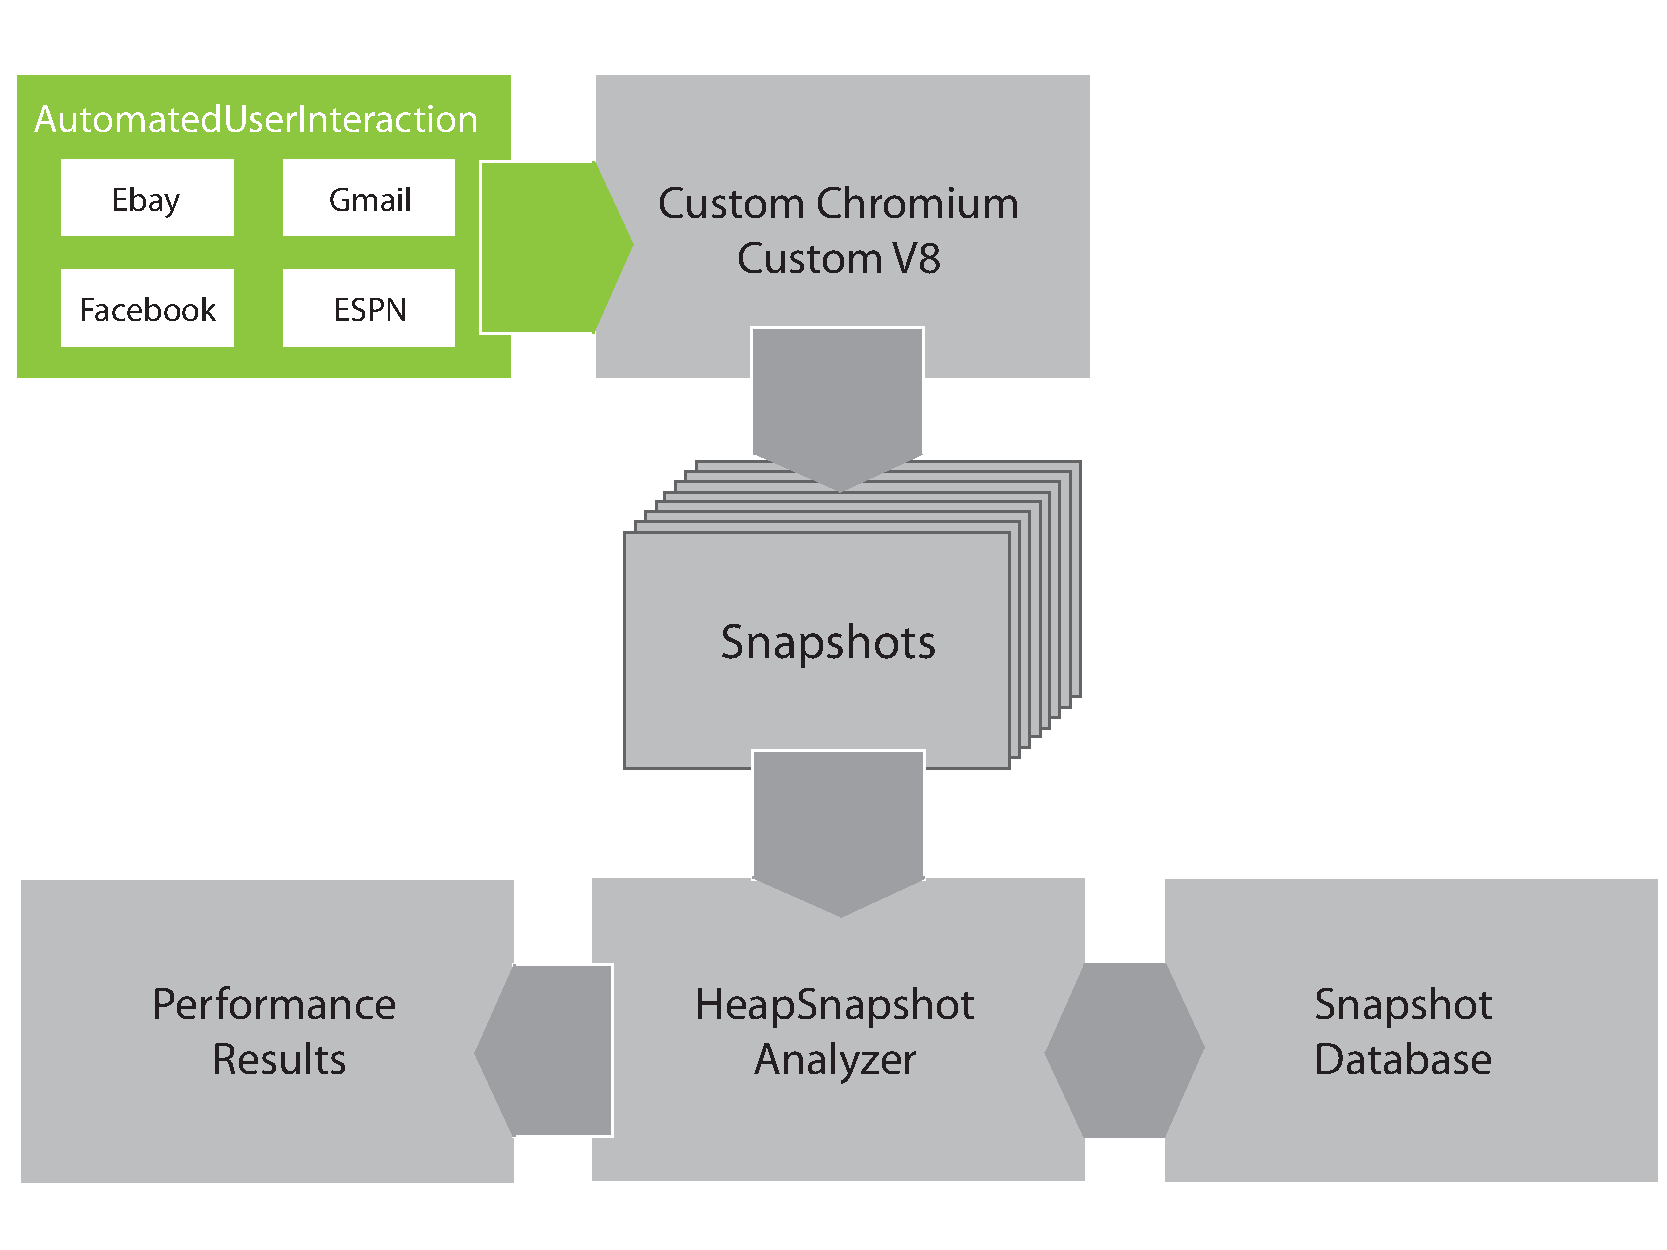
\includegraphics[width=26em]{../imgs/solution_h_1.pdf}
\end{frame}

\subsubsection{AutomatedUserInteraction}
\begin{frame}
	\frametitle{AutomatedUserInteraction}
	\begin{itemize}
		\item Java application
		\item SeleniumHQ framework for automated user interaction
		\begin{itemize}
			\item \href{http://www.seleniumhq.org/}{http://www.seleniumhq.org}
		\end{itemize}
		\item Web applications
		\begin{itemize}
			\item \textbf{News:} CNN, ESPN, The Economist
			\item \textbf{Email:} Gmail, Hotmail
			\item \textbf{Shops:} Ebay, Amazon
			\item \textbf{Maps:} Google, Bing
			\item \textbf{Search:} Google, Bing
			\item \textbf{Social:} Facebook, Google Plus
		\end{itemize}
	\end{itemize}
\end{frame}
	
\begin{frame}
	\frametitle{Step \theStepCounter: Heap model}		
	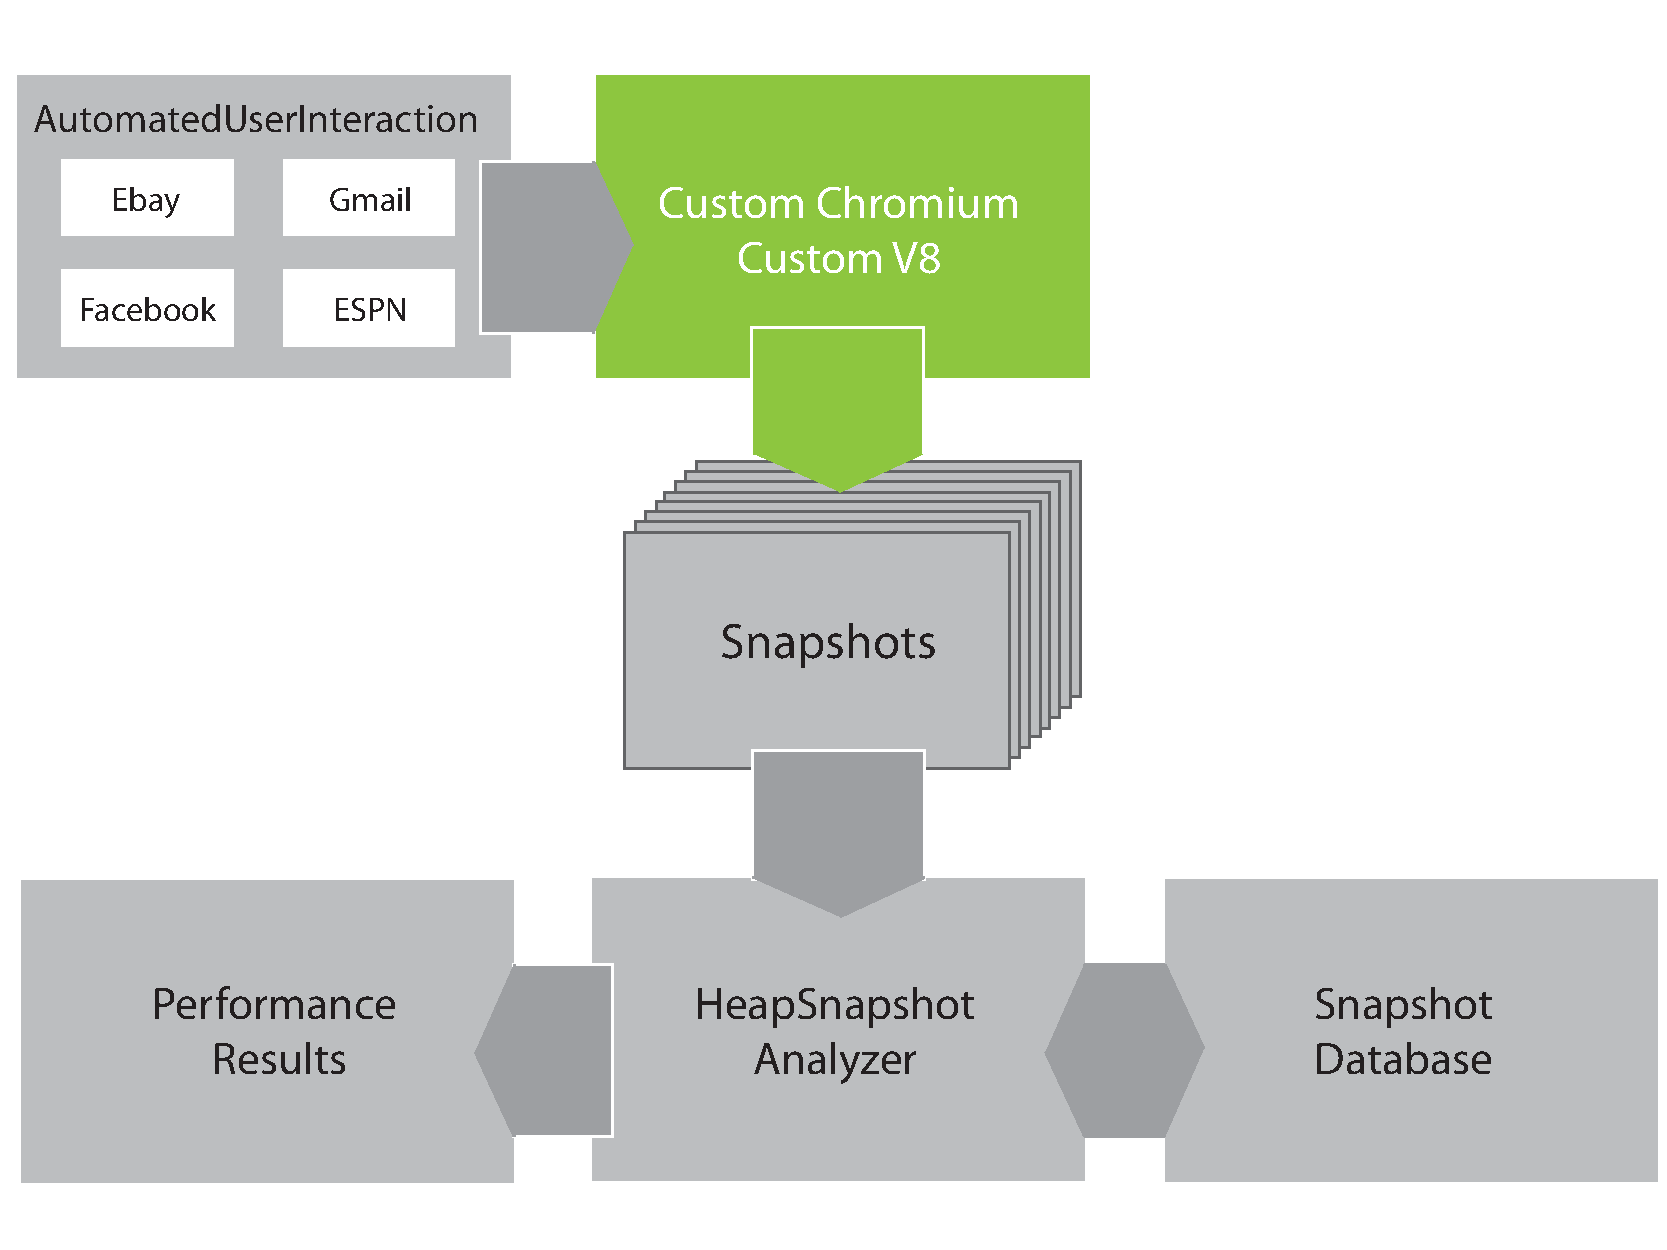
\includegraphics[width=26em]{../imgs/solution_h_2.pdf}
\end{frame}

\subsubsection{Customizations}
\begin{frame}
	\frametitle{Customizations}
	%\begin{columns}
	%	\begin{column}{.55\linewidth}
			Custom Chromium binary
			\begin{itemize}
				\item Used flags
				\begin{itemize}
					\item \texttt{no\_sandbox} 						% Disables the sandbox for all process types that are normally sandboxed.
				\end{itemize}
			\end{itemize}
			
			Custom V8 binary
			\begin{itemize}
				\item New flags
				\begin{itemize}
					\item \texttt{automatic\_heap\_snapshots} 		% create heap snapshot automatically every heap-snapshot-interval KBs
					\item \texttt{heap\_snapshot\_interval} 		% heap snapshot interval in KB
					\item \texttt{heap\_snapshot\_prefix} 			% prefix for the .heapsnapshot files
				\end{itemize}
				\item Used flags
				\begin{itemize}
					\item \texttt{gc\_interval} 					% garbage collect after n allocations
				\end{itemize}
			\end{itemize}
	%	\end{column}
	%	\begin{column}{.35\linewidth}			
	%		\includegraphics<1>[width=9em]{../imgs/chromium_v.pdf}
	%	\end{column}
	%\end{columns}
\end{frame}
	
\begin{frame}
	\frametitle{Step \theStepCounter: Heap model}		
	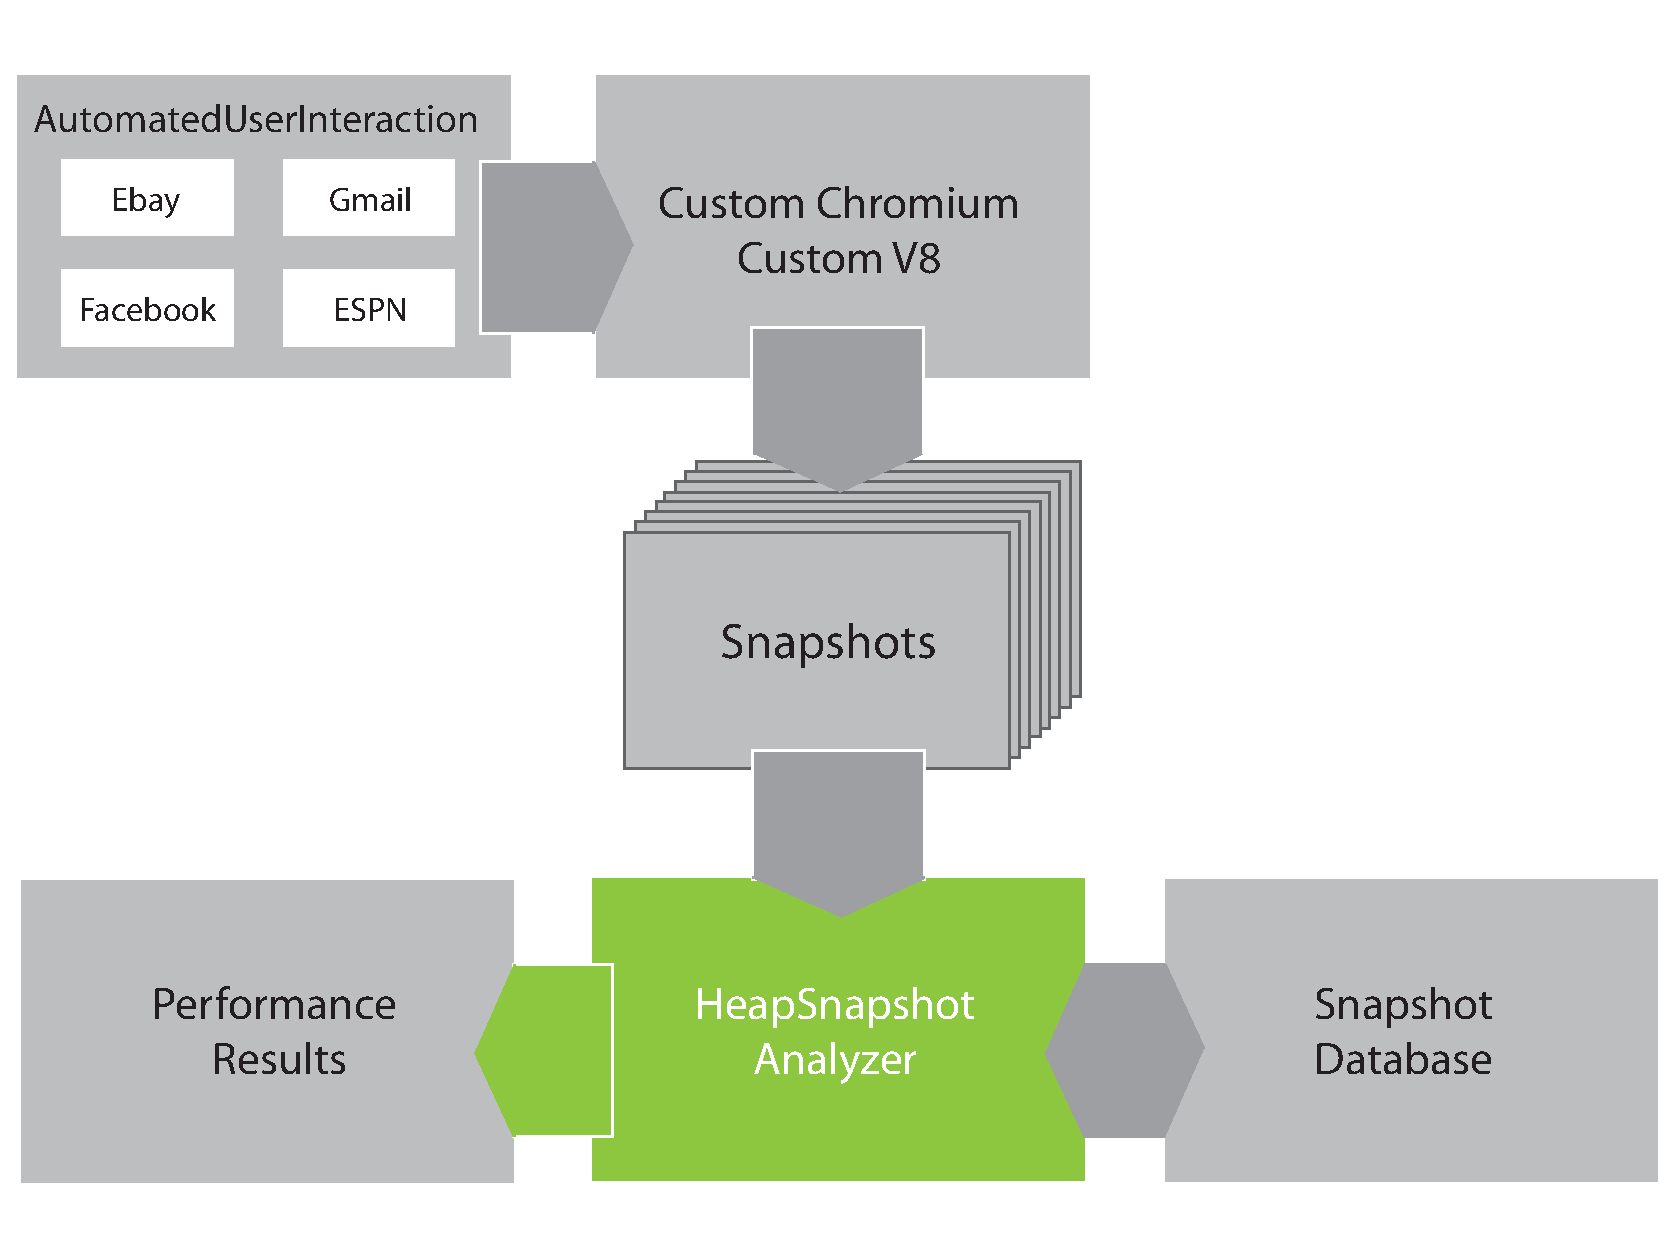
\includegraphics[width=26em]{../imgs/solution_h_3.pdf}
\end{frame}
	
\subsubsection{HeapSnapshotAnalyzer}
\begin{frame}
	\frametitle{HeapSnapshotAnalyzer}
	\begin{itemize}
		\item Java application
		\item PostgreSQL 9.3
		\item Write snapshots into DB
			
		\pause
			
		\item Heap graph
		\begin{itemize}
			 \item Number of leafs
			 \item Number of nodes
			 \item Number of edges
			 \item Number of strongly connected components
		\end{itemize}
			
		\pause 
			
		\item Node characteristics
		\begin{itemize} 
			 \item In-degree
			 \item Out-degree
			 \item Root distance
			 \item Node size 
		\end{itemize}
	\end{itemize} 
\end{frame}
	
\begin{frame}
	\frametitle{Step \theStepCounter: Heap model}		
	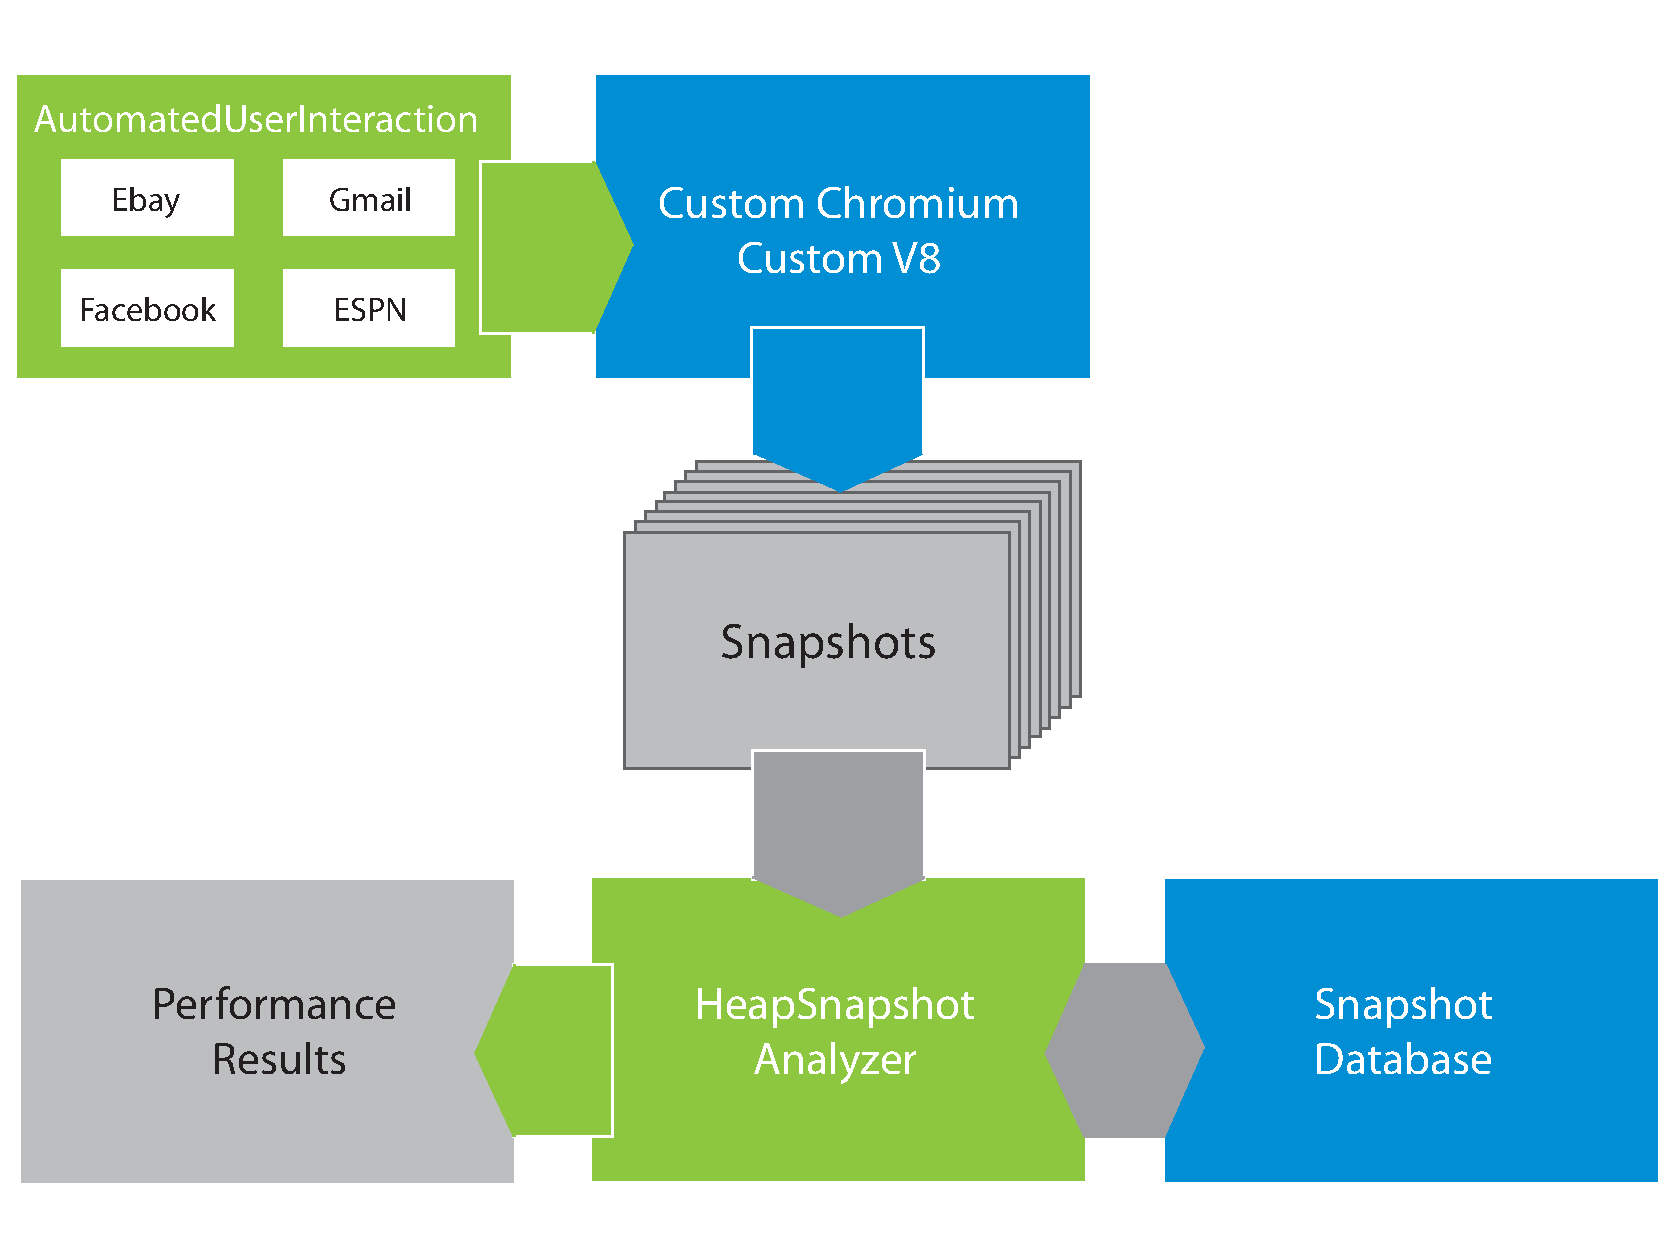
\includegraphics[width=26em]{../imgs/solution_h.pdf}
\end{frame}
	
\stepcounter{StepCounter}
\subsection{Step \theStepCounter: JavaScript mutator}
\begin{frame}
	\frametitle{Step \theStepCounter: JavaScript mutator}
%		Develop a universal JavaScript mutator based on the real web application analyzation results.  
	Develop a 
	\begin{itemize}
		\item Universal JavaScript mutator
		\item Based on the original ACDC implementation.
	\end{itemize}
		
	\pause
		
	Extend this mutator
	\begin{itemize}
		\item With special features for garbage collector measurements
		\item Based on the analysis results simulate
		\begin{itemize}
			\item real web applications and
			\item corner cases. 
		\end{itemize}
	\end{itemize}
\end{frame}
	%-------------------------------------------------------------------
% bachelor thesis - presentation
%
% topic: ACDC4JS - How to analyze a JavaScript garbage collector
%
% create by: Mario Preishuber
% create date: 2014, Jan 01.
%-------------------------------------------------------------------
\section{Experiments}

%\begin{frame}
%	\frametitle{Content}
%	\setcounter{tocdepth}{2}
%	\tableofcontents[currentsection]
%\end{frame}

\begin{frame}
	\frametitle{Experiments}
	\begin{itemize}
		\item Step 1: Simple but artificial mutator
		\item Step 2: Obtaining a realistic heap model
		\item Step 3: Developing a realistic JavaScript mutator (TODO)
	\end{itemize}
\end{frame}

\newcounter{StepCounter}
\stepcounter{StepCounter}

\subsection{Step \theStepCounter: Simple but artificial mutator}
\begin{frame}
	\frametitle{Step \theStepCounter: Simple but artificial mutator}
	\begin{itemize}
		\item Get information about the garbage collector
		\begin{itemize}
			\item Collection frequency %cycle
			\item Quantity of collected memory
			\item Number of collected objects
		%	\item type of garbage collection
		\end{itemize}
		
		\smallskip
		\pause
			
		\item Prepare a simple mutator
		\begin{itemize}
			\item Number of allocated objects
			\item Number of live objects
			\item Size of an object
		\end{itemize}
			
		\smallskip
		\pause
			
		\item Wrap system measurements
		\begin{itemize}
			\item Execution time
			\item Real memory (resident set size ... rss) 
		\end{itemize}
	\end{itemize}
\end{frame}
\begin{frame} 
	\frametitle{Step \theStepCounter: Measurements - allocation only}
	\begin{center}
		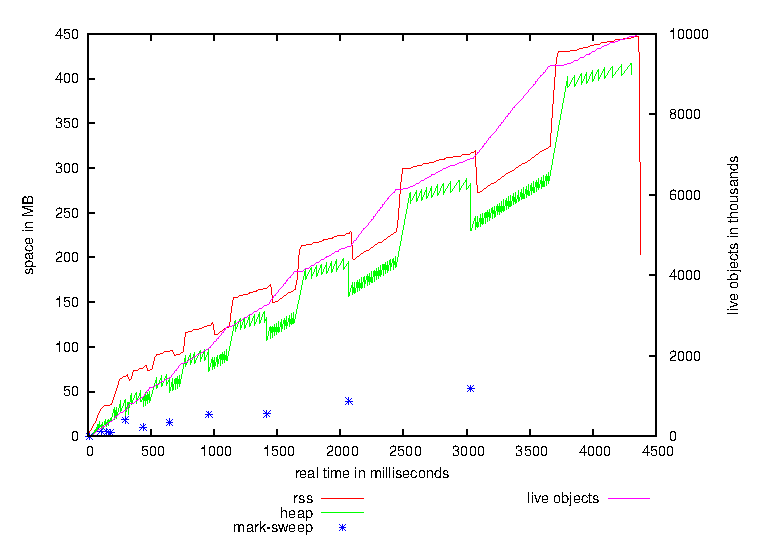
\includegraphics[width=.9\textwidth]{../plots/keep_all_obj_rss_heap_mas_obj_time.eps}
	\end{center}
\end{frame}
\begin{frame} 
	\frametitle{Step \theStepCounter: Measurements - execution time}
	\begin{center}
		\includegraphics[width=.9\textwidth]{../plots/acdc_multi_exec_time.eps}
	\end{center}
\end{frame}
	
\stepcounter{StepCounter}
\subsection{Step \theStepCounter: Obtaining a realistic heap model}
\begin{frame}
	\frametitle{Step \theStepCounter: Obtaining a realistic heap model}
	\begin{itemize}
		\item Important for mutator implementation
		\item Customizations
		\begin{itemize}
			\item Custom Chromium binary
			\item Custom V8 binary
		\end{itemize}
			
		\pause
			
		\item Tools for JavaScript heap analysis
		\begin{itemize}
			\item AutomatedUserInteraction
			\item HeapSnapshotAnalyzer
		\end{itemize}
	\end{itemize}
\end{frame}
	
\begin{frame}
	\frametitle{Step \theStepCounter: Obtaining a realistic heap model}		
	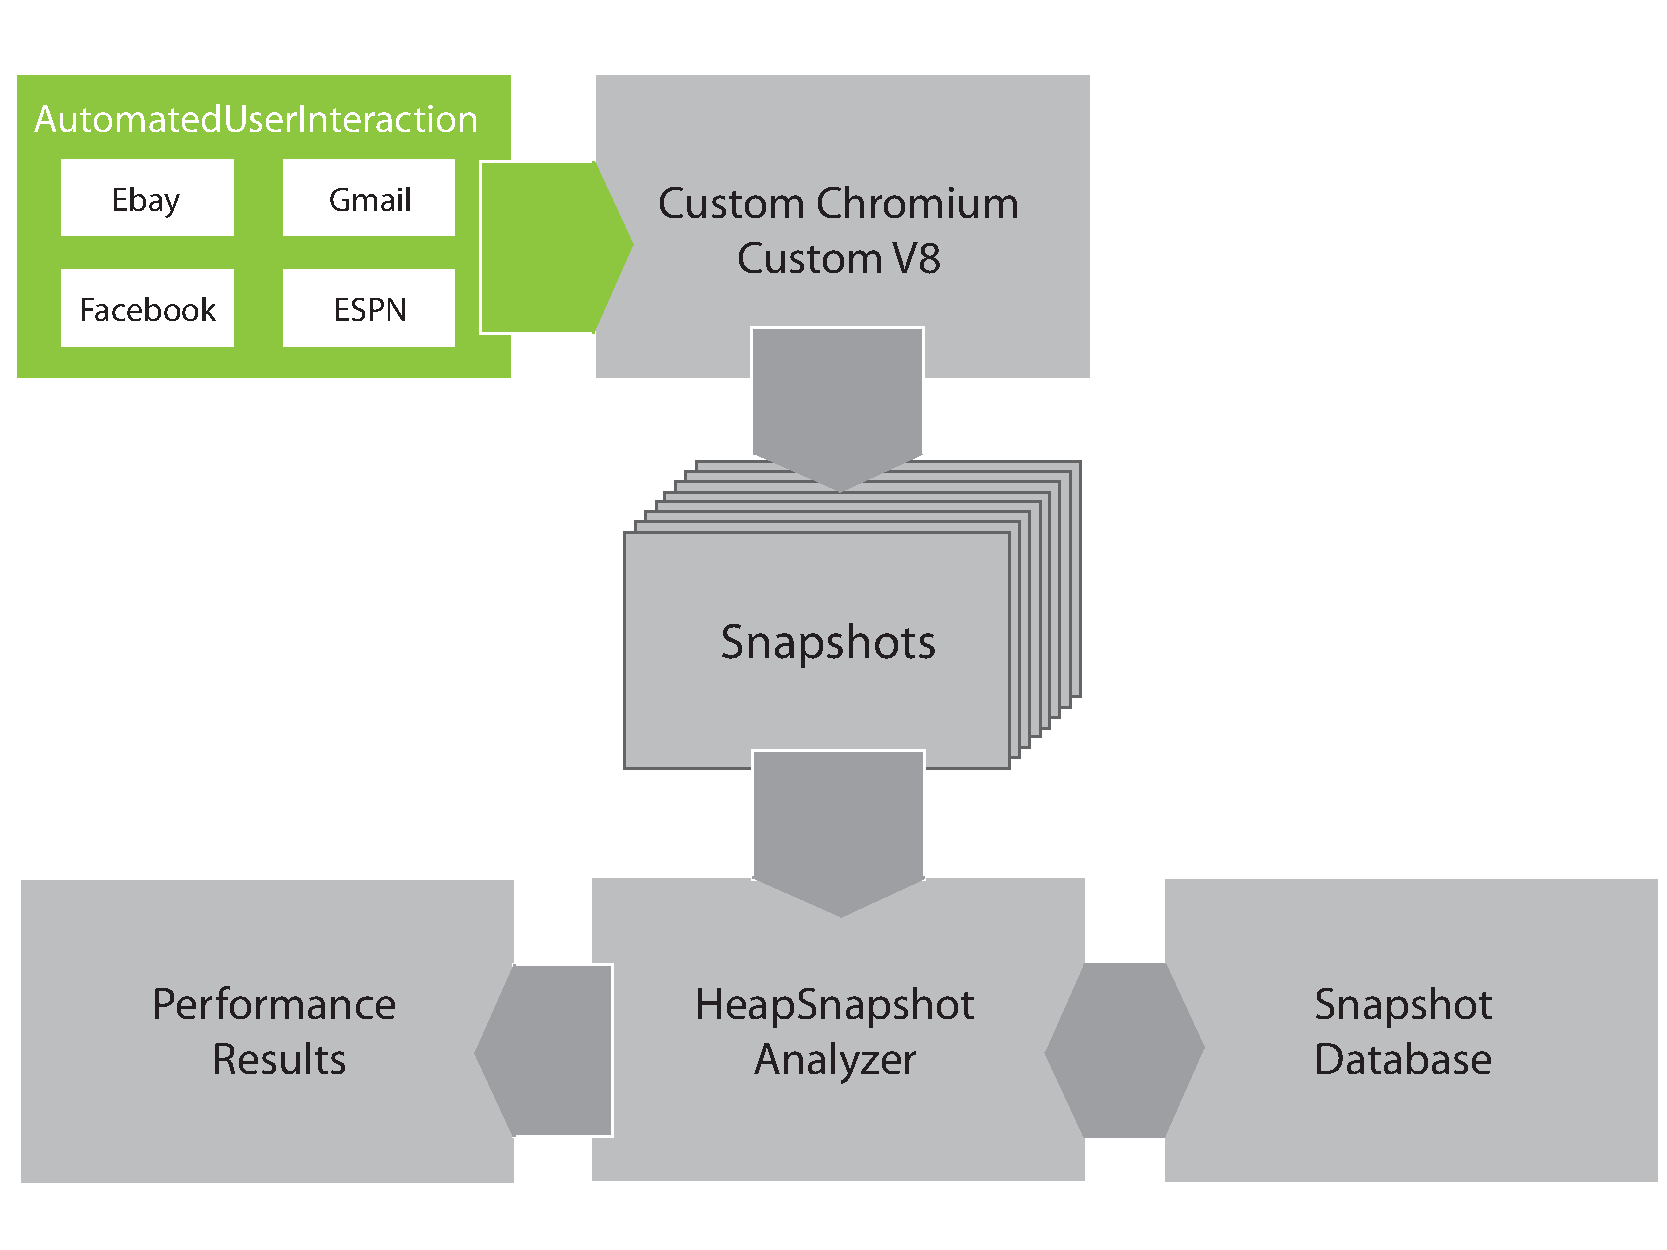
\includegraphics[width=26em]{../imgs/solution_h_1.pdf}
\end{frame}

\subsubsection{AutomatedUserInteraction}
\begin{frame}
	\frametitle{AutomatedUserInteraction}
	\begin{itemize}
		\item Java application
		\item SeleniumHQ framework for automated user interaction
		\begin{itemize}
			\item \href{http://www.seleniumhq.org/}{http://www.seleniumhq.org}
		\end{itemize}
		\item Web applications
		\begin{itemize}
			\item \textbf{News:} CNN, ESPN, The Economist
			\item \textbf{Email:} Gmail, Hotmail
			\item \textbf{Shops:} Ebay, Amazon
			\item \textbf{Maps:} Google, Bing
			\item \textbf{Search:} Google, Bing
			\item \textbf{Social:} Facebook, Google Plus
		\end{itemize}
	\end{itemize}
\end{frame}
	
\begin{frame}
	\frametitle{Step \theStepCounter: Obtaining a realistic heap model}		
	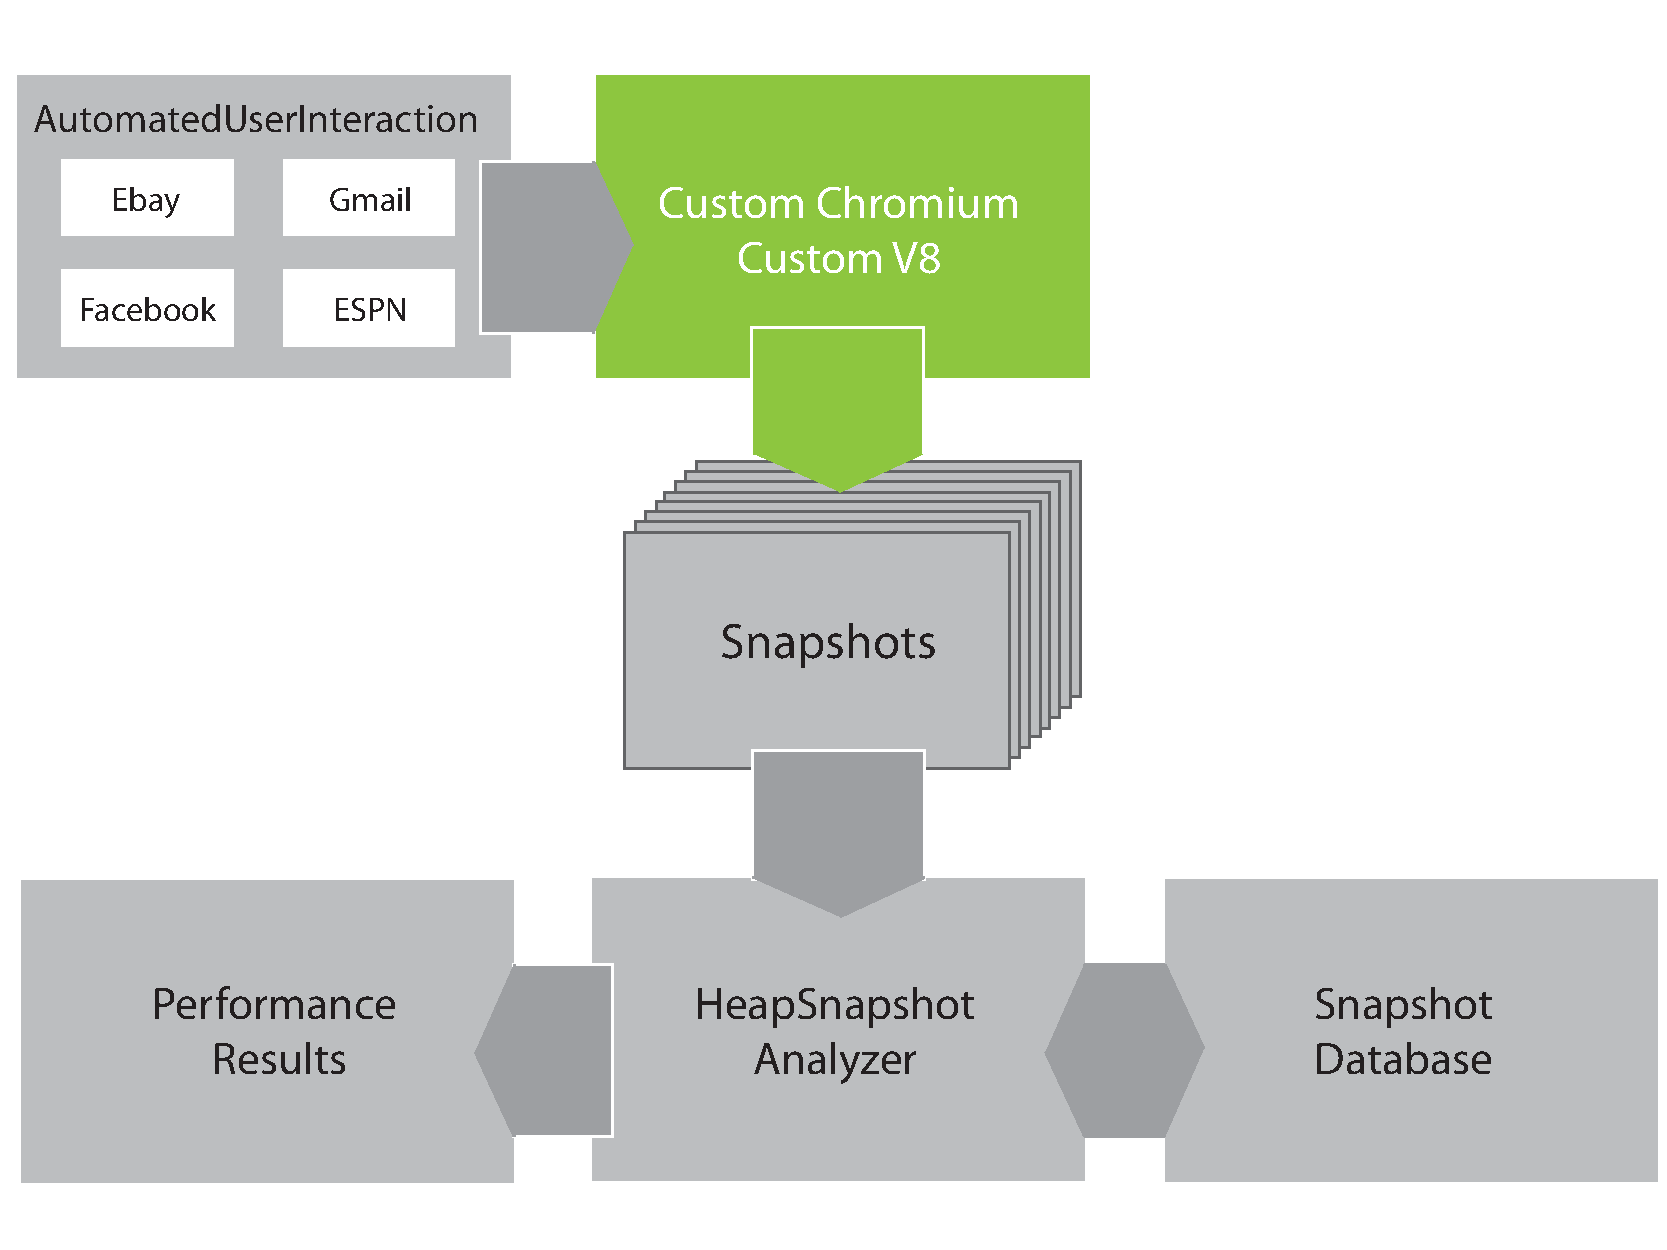
\includegraphics[width=26em]{../imgs/solution_h_2.pdf}
\end{frame}

\subsubsection{Customizations}
\begin{frame}
	\frametitle{Customizations}
	%\begin{columns}
	%	\begin{column}{.55\linewidth}
	%		Custom Chromium binary
	%		\begin{itemize}
	%			\item Used flags
	%			\begin{itemize}
	%				\item \texttt{no\_sandbox} 						% Disables the sandbox for all process types that are normally sandboxed.
	%			\end{itemize}
	%		\end{itemize}
			
			Custom V8 binary
			\begin{itemize}
				\item New flags
				\begin{itemize}
					\item \texttt{automatic\_heap\_snapshots} 		% create heap snapshot automatically every heap-snapshot-interval KBs
					\item \texttt{heap\_snapshot\_interval} 		% heap snapshot interval in KB
					\item \texttt{heap\_snapshot\_prefix} 			% prefix for the .heapsnapshot files
				\end{itemize}
				\item Used flags
				\begin{itemize}
					\item \texttt{gc\_interval} 					% garbage collect after n allocations
				\end{itemize}
			\end{itemize}
	%	\end{column}
	%	\begin{column}{.35\linewidth}			
	%		\includegraphics<1>[width=9em]{../imgs/chromium_v.pdf}
	%	\end{column}
	%\end{columns}
\end{frame}
	
\begin{frame}
	\frametitle{Step \theStepCounter: Obtaining a realistic heap model}		
	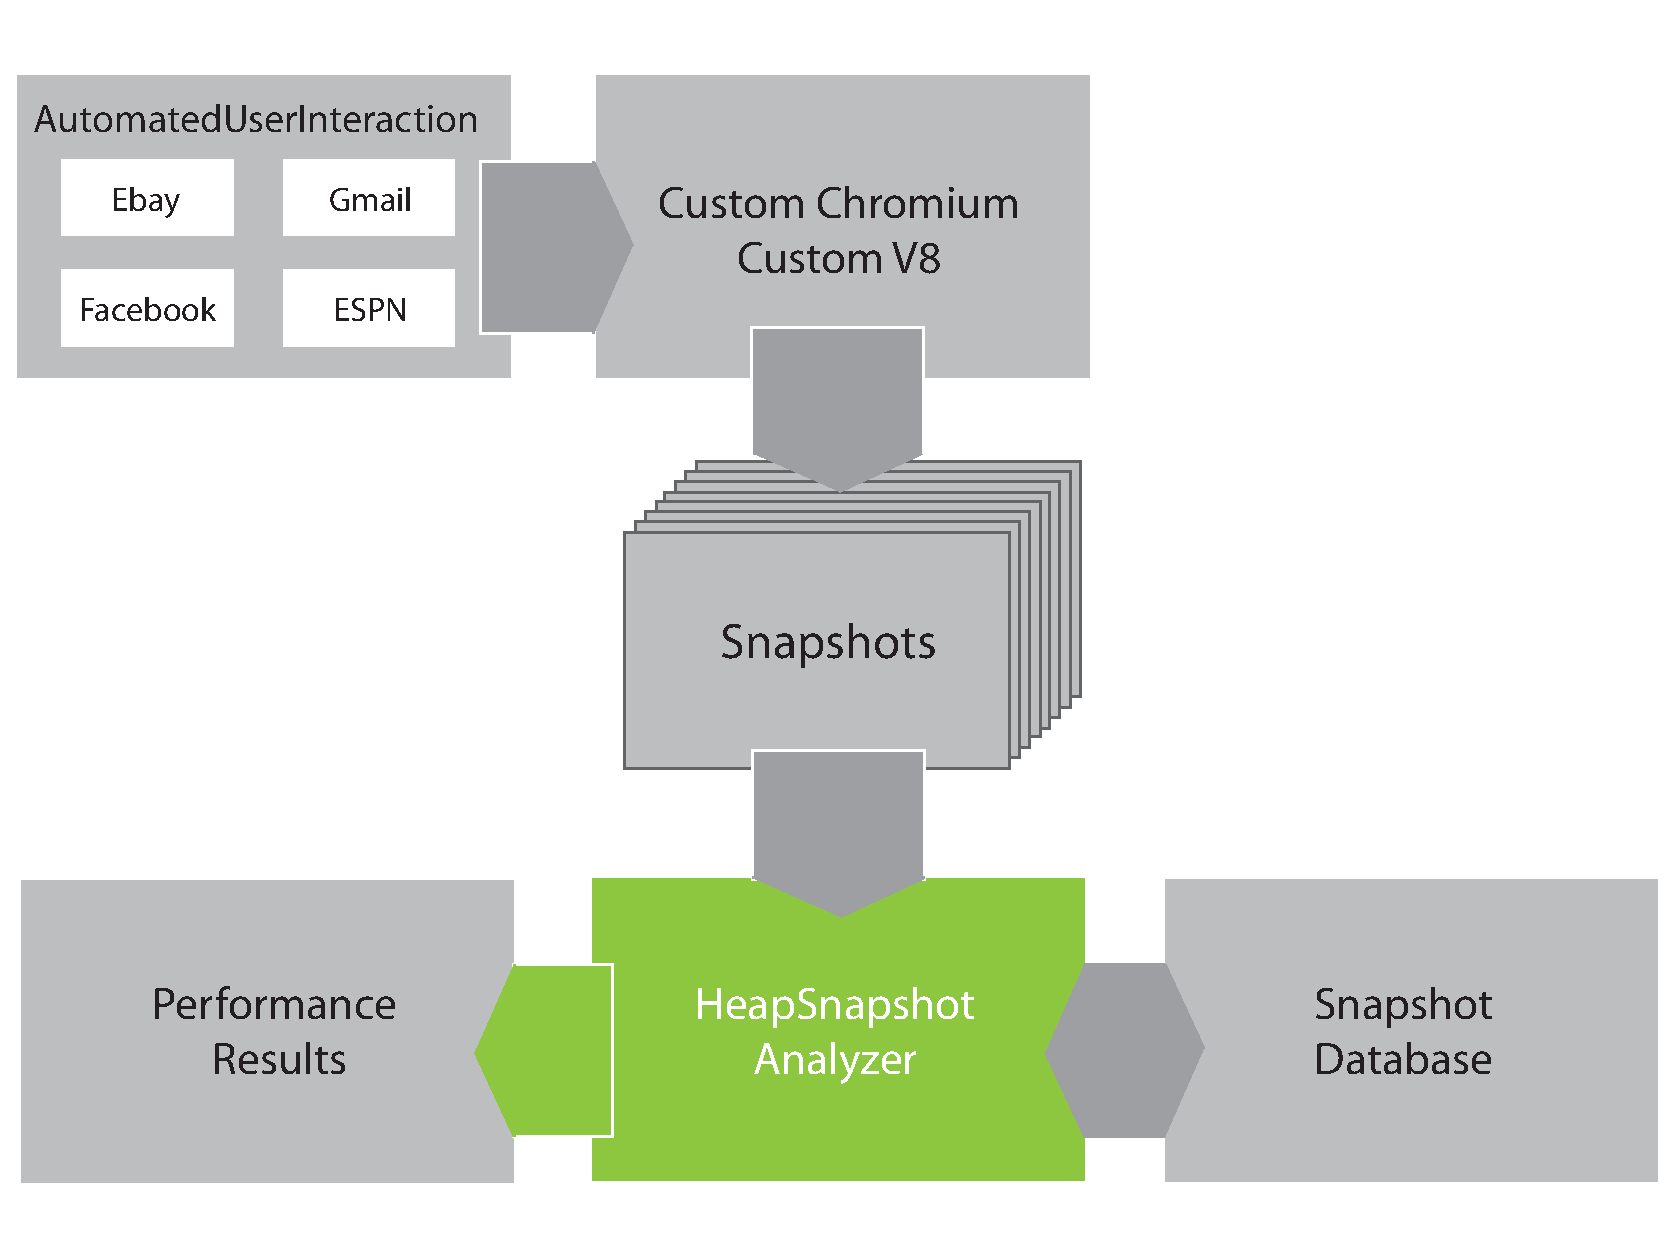
\includegraphics[width=26em]{../imgs/solution_h_3.pdf}
\end{frame}
	
\subsubsection{HeapSnapshotAnalyzer}
\begin{frame}
	\frametitle{HeapSnapshotAnalyzer}
	\begin{itemize}
		\item Java application
		\item PostgreSQL 9.3
		\item Write snapshots into database
			
		\pause
			
		\item Heap graph
		\begin{itemize}
			 \item Number of leafs
			 \item Number of nodes
			 \item Number of edges
			 \item Number of strongly connected components
		\end{itemize}
			
		\pause 
			
		\item Node characteristics
		\begin{itemize} 
			 \item In-degree
			 \item Out-degree
			 \item Root distance
			 \item Node size 
		\end{itemize}
	\end{itemize} 
\end{frame}
	
%\begin{frame}
%	\frametitle{Step \theStepCounter: Obtaining a realistic heap model}		
%	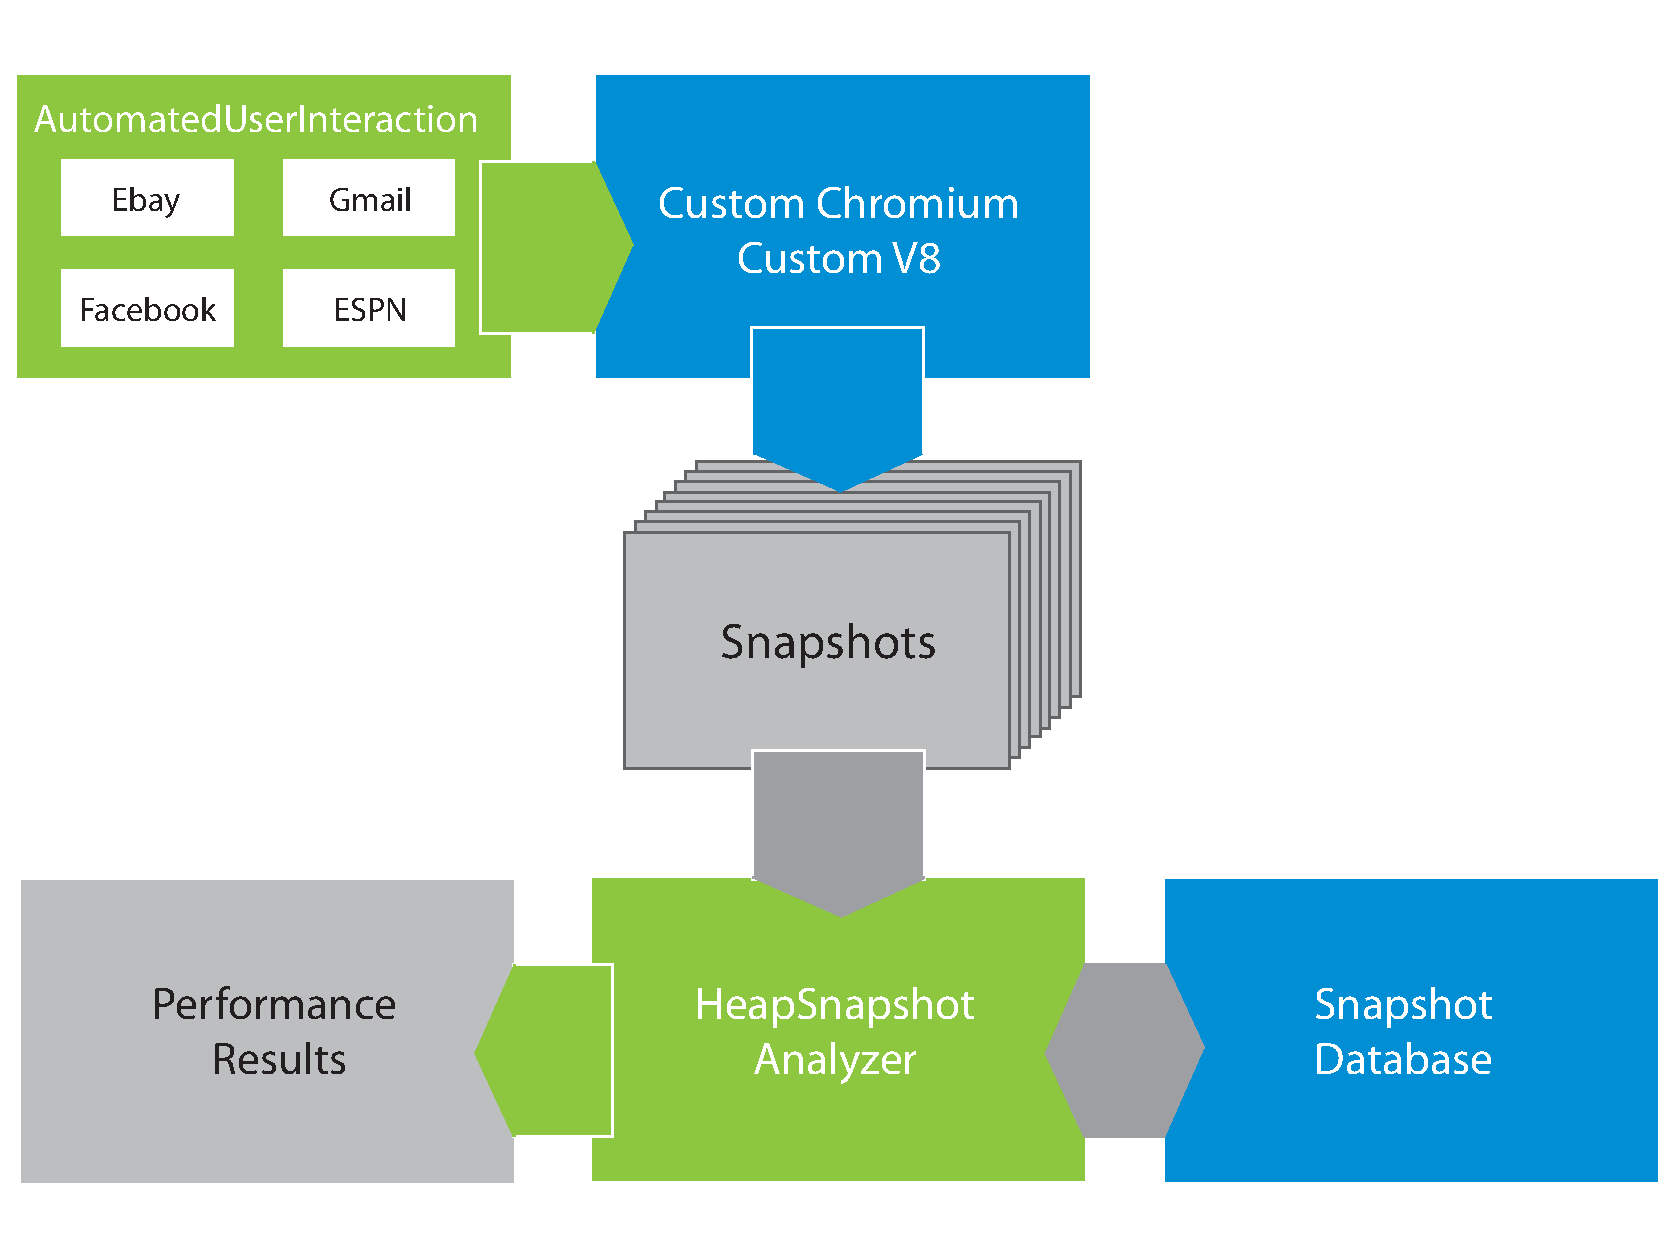
\includegraphics[width=26em]{../imgs/solution_h.pdf}
%\end{frame}
	
\stepcounter{StepCounter}
\subsection{Step \theStepCounter: Developing a realistic JavaScript mutator (TODO)}
\begin{frame}
	\frametitle{Step \theStepCounter: Developing a realistic JavaScript mutator (TODO)}
	\begin{center}
		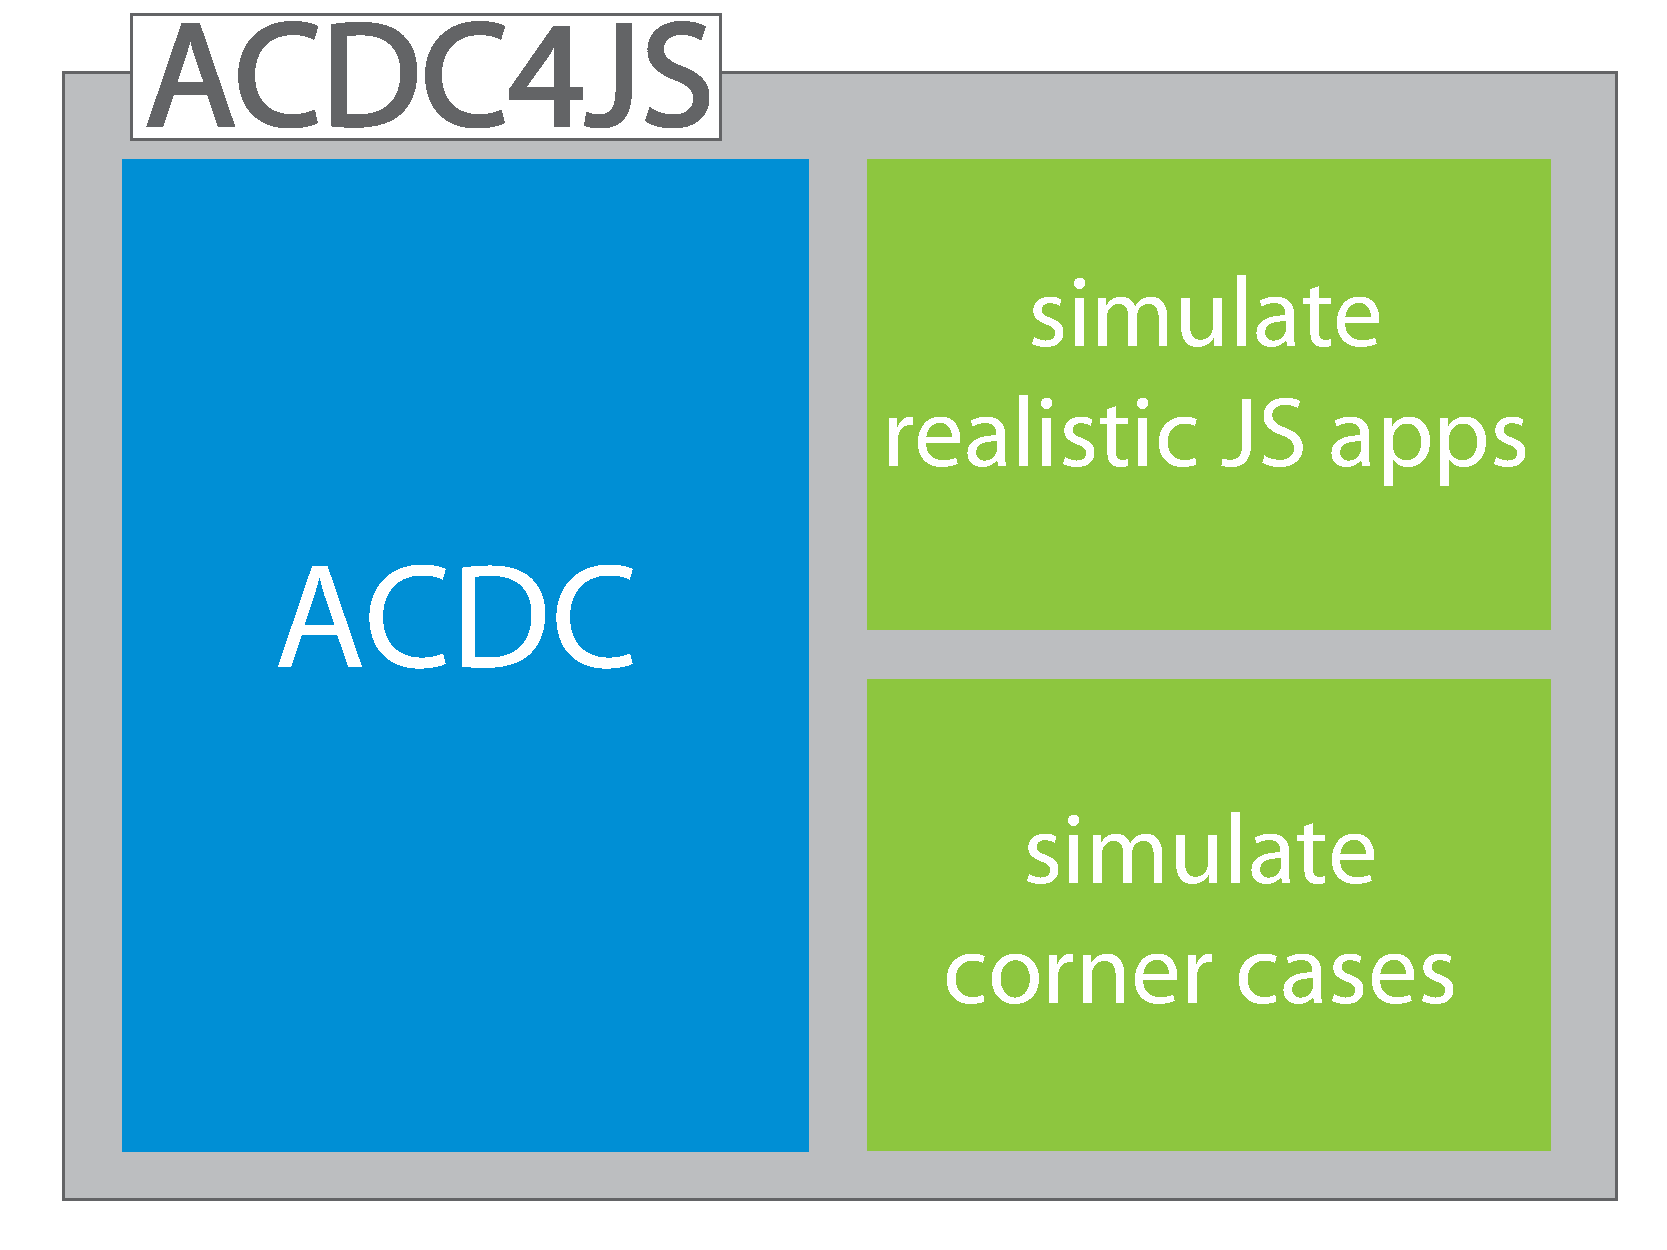
\includegraphics[width=22em]{../imgs/acdc4js.pdf}
	\end{center}
\end{frame}

%		Develop a universal JavaScript mutator based on the real web application analyzation results.  
	% Develop a 
	% \begin{itemize}
	% 	\item Universal JavaScript mutator
	% 	\item Based on the original ACDC implementation
	% \end{itemize}
	% 	
	% \pause
	% 	
	% Extend this mutator
	% \begin{itemize}
	% 	\item With special features for garbage collector measurements
	% 	\item Based on the analysis results simulate
	% 	\begin{itemize}
	% 		\item real web applications and
	% 		\item corner cases 
	% 	\end{itemize}
	% \end{itemize}
	%%-------------------------------------------------------------------
% bachelor thesis - presentation
%
% topic: ACDC4JS - How to analyze a JavaScript garbage collector
%
% create by: Mario Preishuber
% create date: 2014, Jan 01.
%------------------------------------------------------------------- 
\section{Measurement results}
\begin{frame}
	\frametitle{Measurement results}
	\begin{center}
		\includegraphics<1>[width=.9\textwidth]{../plots/keep_all_obj_rss_heap_mas_obj_time.eps}
		\includegraphics<2>[width=.9\textwidth]{../plots/acdc_rss_heap_mas_obj_time.eps}
		\includegraphics<3>[width=.9\textwidth]{../plots/acdc_multi_exec_time.eps}
		%\includegraphics<4>[width=.9\textwidth]{../plots/nodes_edges_leaves.eps}
	\end{center}
\end{frame}
	%%-------------------------------------------------------------------
% bachelor thesis - presentation
%
% topic: ACDC4JS - How to analyze a JavaScript garbage collector
%
% create by: Mario Preishuber
% create date: 2014, Jan 01.
%-------------------------------------------------------------------

\section{Conclusion}
\begin{frame}
	\frametitle{Conclusion}
	Done so far:
	\begin{itemize}
		\item Analyzed garbage collector behavior
		\item Analyzed real web application heap behavior
	\end{itemize}
	To do:
	\begin{itemize}
		\item Complete the implementation of the mutator
	\end{itemize}
\end{frame}	
	\begin{frame}
		\frametitle{Thank you for your attention!}
		\center { \Large{Questions?} }
	\end{frame}
\end{document}